\documentclass[a4paper]{ctexart}
\usepackage[left=2cm, right=2cm, top=2.5cm, bottom=2.2cm]{geometry}

\usepackage{fancyhdr}
\usepackage{graphicx, subfigure}

\usepackage{xcolor}
\IfFileExists{upquote.sty}{\usepackage{upquote}}{}

% \usepackage[sort&compress]{natbib}
% \usepackage{hyperref}
% \hypersetup{unicode, colorlinks=true, linkcolor=black, urlcolor=blue}
\usepackage{booktabs}
\usepackage{multicol}
\usepackage{amsmath}
\usepackage{pgfplots}
\pgfplotsset{compat=1.15}
\usepackage{mathrsfs}
\usetikzlibrary{arrows}

\definecolor{ffzzqq}{rgb}{1,0.6,0}
\definecolor{qqwuqq}{rgb}{0,0.39215686274509803,0}
\definecolor{xdxdff}{rgb}{0.49019607843137253,0.49019607843137253,1}

\title{\textbf{第二次大作业实验报告}}
\author{
zxdclyz
\and
duskmoon314
\and
BobAnkh
}
\date{December 2020}

\ctexset{
    section = {
      format = \zihao{4}\heiti,
      beforeskip = {2ex},
      afterskip = {2ex}
     },
    subsection = {
            format = \zihao{5}\heiti,
            beforeskip = {2ex},
            afterskip = {1ex},
        },
    subsubsection = {
            format = \zihao{5}\songti,
            beforeskip = {2ex},
            afterskip = {1ex},
        },
    appendix = {
            name = {附录}
        }
}

\linespread{1}

\begin{document}

\pagestyle{plain}

\maketitle

\section{原理与实现思路}

\subsection{思路简述}

对于四通道音频信号,首先使用带通滤波和减谱法进行降噪,再以两个麦克风为一组计算六个互相关得到六个角度估计值,最后加权平均得到最终角度结果。

\subsection{具体步骤}
\subsubsection{噪声滤除}
去噪的思路如下:
\begin{enumerate}
    \item 查阅资料可知,女声的频率范围大致在200Hz$-$1200Hz,在考虑泛音的基上,我们使用了200$-$3000Hz的带通FIR滤波器来滤除部分高频和低频噪声;
    \item 通过带通滤波我们滤去了很大一部分噪声,但是通带内仍有一些噪声要处理。对于这部分噪声我们使用了谱减法处理,取音频信号的前一部分作噪声,再对音频分帧计算频谱,然后减去噪声谱,最后逆变换得去噪后的信号。
\end{enumerate}
\centerline{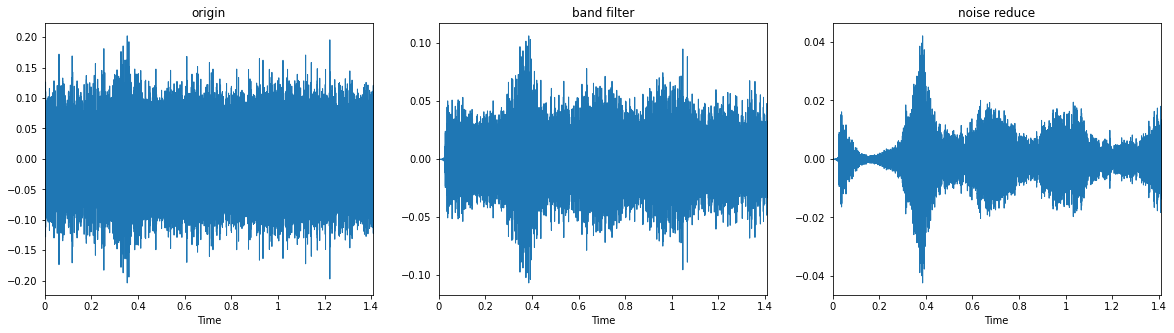
\includegraphics[scale=0.4]{noisereduce.png}}
\subsubsection{分组计算角度}

首先考虑两个麦克风接收平面波的情况。假设两个麦克风接收的平面波与麦克风连线夹角为$\theta$,两个麦克风间距$l$,则与时延对应的距离$d=l \cos{\theta}$,时延$\Delta t = d / v_{\text{声}}$。故可以对两个麦克风接收到的信号计算相关,取最大值和0的距离作为时延,进而求解出角度的估计$\hat{\theta}$。

\centerline{
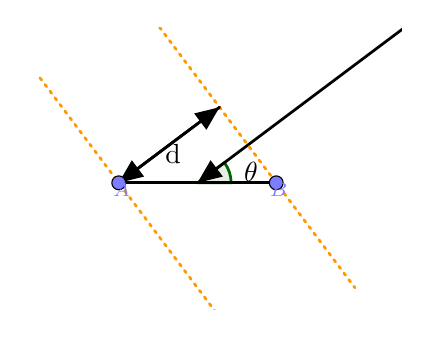
\begin{tikzpicture}[line cap=round,line join=round,>=triangle 45,x=1cm,y=1cm]
\clip(-2.1565127329288574,-1.6077951418802583) rectangle (2.5972756307153873,1.9703710994598864);
\draw [shift={(0,0)},line width=1pt,color=qqwuqq,fill=qqwuqq,fill opacity=0.10000000149011612] (0,0) -- (0:0.4274989535651299) arc (0:36.86989764584402:0.4274989535651299) -- cycle;
\draw [->,line width=1pt] (4,3) -- (0,0);
\draw [line width=1pt,dotted,color=ffzzqq,domain=-2:2] plot(\x,{(--4-4*\x)/3});
\draw [line width=1pt,dotted,color=ffzzqq,domain=-2:2] plot(\x,{(-4-4*\x)/3});
\draw [->,line width=1pt] (-1,0) -- (0.28,0.96);
\draw [->,line width=1pt] (0.28,0.96) -- (-1,0);
\draw (-0.5320167093813638,0.6151994166584218) node[anchor=north west] {d};
\draw (0.4683308419610402,0.38007499219759994) node[anchor=north west] {$\theta$};
\draw [line width=1pt] (-1,0)-- (1,0);
\begin{scriptsize}
\draw [fill=xdxdff] (-1,0) circle (2.5pt);
\draw[color=xdxdff] (-0.963790652482145,0.09151319854113663) node [anchor=north] {$A$};
\draw [fill=xdxdff] (1,0) circle (2.5pt);
\draw[color=xdxdff] (1.0326294606670117,0.09151319854113663) node [anchor=north] {$B$};
\end{scriptsize}
\end{tikzpicture}
}

由于在声音角度与麦克风接近平行的时候arccos的斜率比较大,会放大我们的计算误差,以至于在有些时候得到的$cos\theta$值会超出$-1\sim1$的范围,尽管我们后面会舍去这样的角度,但为了防止特殊情况下由于这里的误差我们没有将它判定为误差较大的角,我们在此对边缘部分对$cos\theta$进行了一个非线性的映射来限制它处于$-1\sim1$的范围并且适当减小了误差。

一共四个麦克风,两个一组可以得到六个角度估计值,即使简单的取平均也可得到比较不错的估计结果。下面介绍我们进一步优化使用的方法。

\subsubsection{角度加权合并}
    
如前所述,因为在计算arccos时对于靠近-1和1的三角函数值所计算出来的角度值误差比较大,所以在使用以上过程得到的6组角度数据时,为小于$15^{\circ}$和大于$165^{\circ}$的角度赋予权值0(即不使用这样的角度来运算最终角度),为$65^{\circ}-115^{\circ}$之间的角度赋予高权值,其余角度赋予低权值,从而加权平均后四舍五入得到最终角度。

\subsubsection{采用多进程并行加速处理}

因为考虑到测试集上需要处理的数据量比较大,为了加速运行,引入了多进程操作。使用标准库中的\texttt{multiprocessing.Pool()}类创建了进程池,来调用多个进程将处理任务映射到多核上并行处理,从而减少总体的处理时间。

\section{结果展示与分析}
使用训练集进行角度估计,结果展示如下:

\begin{table}[h]
    \centering
    \begin{tabular}{ccc|ccc}
        \toprule
        语音序号 & 真实值 & 估计值 & 语音序号 & 真实值 & 估计值         \\
        \midrule
        1 & 315.000  & 315.000 & 8 & 84.000  & 84.000  \\ 
        2 & 358.000  & 358.000  & 9 & 119.000  & 119.000  \\ 
        3 & 107.000  & 107.000  & 10 & 349.000  & 349.000  \\  
        4 & 154.000  & 154.000  & 11 & 218.000  & 218.000  \\ 
        5 & 48.000  & 47.000  & 12 & 107.000  & 107.000  \\ 
        6 & 201.000  & 201.000  & 13 & 297.000  & 297.000  \\ 
        7 & 303.000  & 303.000  & 14 & 109.000  & 109.000  \\
        \bottomrule
    \end{tabular}
\end{table}

可以看到,在训练集上我们的方法的准确性非常好,只有5号语音估计错误,且差错仅$1^{\circ}$。

\section{使用说明与文件清单}

\subsection{使用说明}
\begin{enumerate}

    \item 运行\texttt{setup.py}来安装需要的依赖包。

    \item 以命令行方式运行\texttt{main.py},并使用\texttt{-d}参数来指定测试数据目录(默认值为\textit{test}),完整说明请参见\texttt{-h}参数。例如将测试数据集放在同目录\textit{test}文件夹下,则可使用如下命令行来运行:
    
    \begin{verbatim}
    python main.py -d test
    \end{verbatim}
\end{enumerate}
\subsection{文件清单}

\begin{table}[h]
    \centering
    \caption{\textit{文件清单}}
    \begin{tabular}{ll}
        \toprule
        文件名称         & 说明                       \\
        \midrule
        main.py          & 主程序,按照上述使用说明在命令行中运行  \\
        setup.py         & Python 3.6.12下配置运行环境  \\
        requirements.txt & 依赖库说明文件                   \\
        \bottomrule
    \end{tabular}
\end{table}

\section{总结与反思}
我们在这次实验中最核心的方法仅仅是基于最简单的相关计算,也已经在这个问题上达到了不错的精度,可见相关这一计算工具的强大与实用性。本次实验中降噪部分也对我们的精度提示有不少帮助,这提示了我们对数据进行预处理的重要性。而有关不足,我们认为对于多个mic(圆阵)的整体利用还可以加强,目前只利用了两两mic组合的加权求和。
\end{document}
